% LearnMate -- IEEE conference (4-page) system demonstration paper.
%
% Build:  cd paper
%         pdflatex main && bibtex main && pdflatex main && pdflatex main
%
% Numbers: every benchmark value quoted in the text is a \val{Name} macro defined in
%          tables/numbers.tex, which integrated-backend/eval/tables.py writes from the
%          evaluation result files. If a script has not produced a value yet, it prints ??,
%          so the paper cannot contain a made-up measurement. Generated tables are
%          \input only when their file exists; until then they print "[pending: run eval]".
%
% Page budget: 4 pages including references, and it is full. When eval/tables.py fills
%          Tables II and III, they become several lines longer, so check the page count
%          again afterwards; the easiest space to recover is in the Section IV scenarios.
\documentclass[conference]{IEEEtran}
\IEEEoverridecommandlockouts
\usepackage{cite}
\usepackage{amsmath,amssymb,amsfonts}
\usepackage{graphicx}
\usepackage{booktabs}
\usepackage{textcomp}
\usepackage{xcolor}
\usepackage{url}
\usepackage{tikz}
\usetikzlibrary{positioning,shapes.geometric,arrows.meta,calc}

\IfFileExists{tables/numbers.tex}{% Generated by eval/tables.py -- every number quoted in the text.
\newcommand{\CacheEmbFalseHit}{68.5}
\newcommand{\CacheEmbPrecision}{69.6}
\newcommand{\CacheEntries}{124}
\newcommand{\CacheFalseHit}{23.1}
\newcommand{\CacheLookupMs}{80}
\newcommand{\CachePrecision}{85.0}
\newcommand{\CacheRecall}{71.5}
\newcommand{\CacheTau}{0.70}
\newcommand{\CorpusChunks}{341}
\newcommand{\CorpusDocs}{8}
\newcommand{\CorpusPages}{100}
\newcommand{\HeatARI}{0.562}
\newcommand{\HeatAttribution}{68.9}
\newcommand{\HeatAttributionNear}{74.4}
\newcommand{\HeatClustered}{91.8}
\newcommand{\HeatNMI}{0.829}
\newcommand{\HeatPlanted}{56.2}
\newcommand{\HeatScaleN}{2,000}
\newcommand{\HeatScaleS}{11.1}
\newcommand{\HeatTurns}{480}
\newcommand{\IRLegacyLatency}{54.5}
\newcommand{\IRLegacyNdcg}{0.752}
\newcommand{\IRLegacyRThree}{85.2}
\newcommand{\IRNdcgGainPct}{-0.1}
\newcommand{\IRQueries}{372}
\newcommand{\IRRrfLatency}{62.8}
\newcommand{\IRRrfNdcg}{0.752}
\newcommand{\IRRrfPValue}{0.592}
\newcommand{\IRRrfRThree}{85.2}
\newcommand{\ModeAccuracy}{96.2}
\newcommand{\WorkloadAsks}{480}
\newcommand{\WorkloadFamilies}{126}
\newcommand{\WorkloadQuestions}{504}
\newcommand{\WorkloadStudents}{40}
}{}
\newcommand{\val}[1]{\ifcsname #1\endcsname\csname #1\endcsname\else\textbf{??}\fi}
\newcommand{\tbl}[1]{\IfFileExists{tables/#1.tex}{\input{tables/#1.tex}}%
  {\textit{[pending: run \texttt{python -m eval.tables}]}}}
\newcommand{\sys}{LearnMate}

\begin{document}

\title{LearnMate: A Fully Local Study Assistant\\That Scales from One Student to a Whole Class}

% TODO(authors): replace with the full names, departments and emails of every author.
\author{\IEEEauthorblockN{Dinura Ginige}
\IEEEauthorblockA{\textit{Dept. of Computer Science} \\
\textit{University (TODO)}\\
Colombo, Sri Lanka \\
dinura1ginige@gmail.com}
\and
\IEEEauthorblockN{2\textsuperscript{nd} Given Name Surname}
\IEEEauthorblockA{\textit{Dept. name of organization} \\
\textit{Name of organization}\\
City, Country \\
email address}
\and
\IEEEauthorblockN{3\textsuperscript{rd} Given Name Surname}
\IEEEauthorblockA{\textit{Dept. name of organization} \\
\textit{Name of organization}\\
City, Country \\
email address}
\and
\IEEEauthorblockN{4\textsuperscript{th} Given Name Surname}
\IEEEauthorblockA{\textit{Dept. name of organization} \\
\textit{Name of organization}\\
City, Country \\
email address}
}

\maketitle
% Forces "et al." after two author names (see the IEEEtranBSTCTL entry in
% references.bib), which keeps the reference list inside the 4-page limit.
\bstctlcite{IEEEexample:BSTcontrol}

\begin{abstract}
Study assistants based on local language models keep students' notes and questions on hardware
controlled by the institution. However, they are usually designed for one student at a time:
generating one grounded answer can occupy the machine long enough for a class to form a queue, and
the system does not learn from the class as a whole. We demonstrate \sys{}, an open-source
retrieval-augmented study assistant in which all models run locally. A student uploads course notes
and receives grounded chat with page citations, together with practice questions, key points and
summaries, each checked by a second model before use. Since each document is stored once using its
content hash, students who share the same lecture notes also share one index and, during revision,
often ask similar questions. \sys{} uses this sharing through four mechanisms: hybrid dense and
BM25 retrieval combined inside the vector database; a verified answer cache that reuses a
judge-approved answer only when a cross-encoder confirms that two students asked the same question;
a lease-based job queue connected to a worker pool and continuously batched model servers; and
confusion mining, which groups student questions by pages of the shared notes while applying a
$k$-anonymity floor. In an end-to-end run, reuse answered a repeated question about two orders of
magnitude faster than generating it again on the same machine, and a worker killed during an answer
had its job recovered by another worker.
\end{abstract}

\begin{IEEEkeywords}
retrieval-augmented generation, local language models, semantic caching, hybrid retrieval,
learning analytics, educational technology
\end{IEEEkeywords}

\section{Introduction}

Large language models can explain, quiz and summarise course material when needed, while
retrieval-augmented generation (RAG) \cite{lewis2020rag} allows them to answer using a student's own
notes instead of only their learned knowledge, reducing confident unsupported answers. Running the
models locally keeps the notes and questions private, which is important for institutions that
cannot send student data to third parties. The trade-off is speed and scalability: on a CPU, a
3B-parameter model generates one grounded answer much more slowly than a class can wait, and a
single model instance handles only one request at a time.

\sys{} started as a single-student assistant: a student uploads a PDF, Word, PowerPoint or \LaTeX{}
file and can ask questions or generate practice material from it, with a second model checking every
output first. One implementation detail makes larger-scale use possible. Documents are identified
by the SHA-256 hash of their bytes. Therefore, when thirty students upload the same lecture notes,
the file is stored, cleaned, chunked and embedded \emph{once}, and all thirty students use the same
document. During revision for the same exam, they also tend to ask similar questions using different
wording.

This paper presents the working system and four mechanisms that turn one shared document into
shared capacity: \textbf{hybrid retrieval inside the vector database}
(Section~\ref{sec:retrieval}); a \textbf{verified answer cache} (Section~\ref{sec:cache}), where
an accepted answer is reused only after a cross-encoder confirms that the two questions match; a
\textbf{lease queue and worker pool} (Section~\ref{sec:serving}), which allows multiple workers to
serve the class without losing a question when a worker crashes; and \textbf{confusion mining}
(Section~\ref{sec:mining}), which creates a per-page map showing where the shared notes cause
difficulty. All models run locally: Qwen2.5-3B-Instruct \cite{qwen2025qwen25} generates answers,
Llama-3.2-3B-Instruct \cite{grattafiori2024llama3} grades them, and MiniLM models embed and rerank
passages. The generator and judge use different model families on purpose: when the judge shares the
generator's weights, it may rate the generator's own style highly, causing the quality gate to lose
its usefulness. Code, the evaluation harness and a screencast are available.\footnote{TODO(authors): repository URL
and demonstration video link.}

\begin{figure*}[t]
\centering
% System architecture, drawn in TikZ so the paper needs no external image.
% Two rows on purpose: a flat figure costs a 4-page paper much less vertical space than a
% square one. Row 1 is the path of one request; row 2 is the stores, model servers and miner.
% Blue boxes are the four classroom-scale components (Sections III-B to III-E).
\resizebox{\textwidth}{!}{%
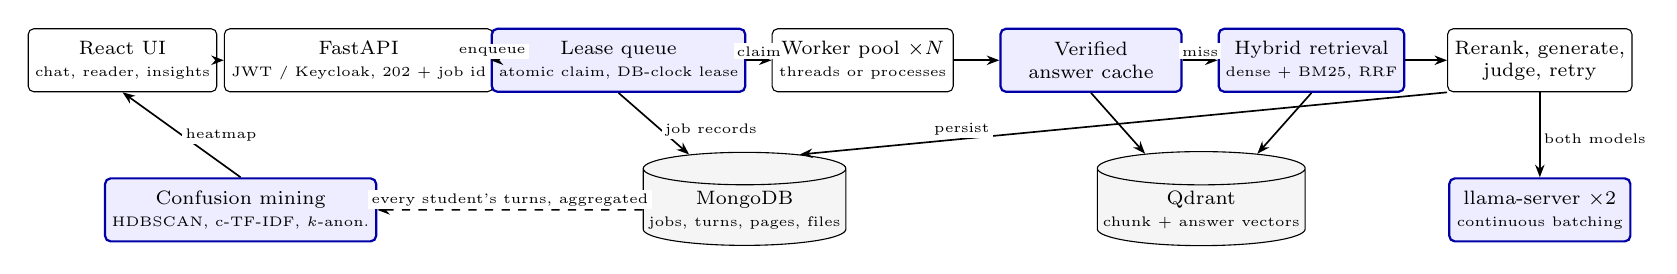
\begin{tikzpicture}[
    font=\scriptsize,
    box/.style={draw, rounded corners=2pt, align=center, minimum height=0.8cm,
                minimum width=2.3cm, inner sep=2.5pt, fill=white},
    new/.style={box, draw=blue!65!black, fill=blue!7, thick},
    store/.style={draw, cylinder, shape border rotate=90, aspect=0.16, align=center,
                  minimum height=0.9cm, minimum width=2.1cm, inner sep=2pt, fill=gray!8},
    arr/.style={-{Stealth[length=1.6mm]}, semithick},
    lbl/.style={font=\tiny, inner sep=1.2pt, fill=white},
]
% Row 1: one request, left to right.
\node[box] (ui)    at (0, 0)      {React UI\\\tiny chat, reader, insights};
\node[box] (api)   at (3.0, 0)    {FastAPI\\\tiny JWT / Keycloak, 202 + job id};
\node[new] (queue) at (6.3, 0)    {Lease queue\\\tiny atomic claim, DB-clock lease};
\node[box] (work)  at (9.4, 0)    {Worker pool $\times N$\\\tiny threads or processes};
\node[new] (cache) at (12.3, 0)   {Verified\\answer cache};
\node[new] (retr)  at (15.1, 0)   {Hybrid retrieval\\\tiny dense + BM25, RRF};
\node[box] (gen)   at (18.0, 0)   {Rerank, generate,\\judge, retry};

% Row 2: what row 1 talks to.
\node[new]   (mine)   at (1.5, -1.9)   {Confusion mining\\\tiny HDBSCAN, c-TF-IDF, $k$-anon.};
\node[store] (mongo)  at (7.9, -1.9)   {MongoDB\\\tiny jobs, turns, pages, files};
\node[store] (qdrant) at (13.7, -1.9)  {Qdrant\\\tiny chunk + answer vectors};
\node[new]   (llama)  at (18.0, -1.9)  {llama-server $\times 2$\\\tiny continuous batching};

% Row 1 edges.
\draw[arr] (ui) -- (api);
\draw[arr] (api) -- node[lbl, above] {enqueue} (queue);
\draw[arr] (queue) -- node[lbl, above] {claim} (work);
\draw[arr] (work) -- (cache);
\draw[arr] (cache) -- node[lbl, above] {miss} (retr);
\draw[arr] (retr) -- (gen);

% Down to the stores and servers.
\draw[arr] (queue.south) -- node[lbl, pos=0.6, right] {job records} (mongo.north west);
\draw[arr] (gen.south) -- node[lbl, pos=0.55, right] {both models} (llama.north);
\draw[arr] (gen.south west) -- node[lbl, pos=0.75, above] {persist} (mongo.north east);
\draw[arr] (cache.south) -- (qdrant.north west);
\draw[arr] (retr.south) -- (qdrant.north east);

% Mining reads every student's turns and feeds the UI.
\draw[arr, dashed] (mongo.west) -- node[lbl, above] {every student's turns, aggregated} (mine.east);
\draw[arr] (mine.north) -- node[lbl, right] {heatmap} (ui.south);
\end{tikzpicture}}

\caption{\sys{} architecture. A chat turn is processed as a background job: the API returns \texttt{202} with
a job id, a worker claims the job under a lease and runs the turn graph (rewrite $\rightarrow$
cache lookup $\rightarrow$ hybrid retrieval $\rightarrow$ rerank $\rightarrow$ generate
$\rightarrow$ judge $\rightarrow$ persist $\rightarrow$ cache store). Blue boxes show the four
classroom-scale components; the dashed edge is the mining path, which reads all student
turns and produces one aggregate heatmap.}
\label{fig:arch}
\end{figure*}

\section{Related Work}

Hybrid lexical-dense retrieval and fusion methods are well studied \cite{cormack2009rrf}, as are
learned sparse representations \cite{formal2021splade}. \sys{} focuses on an engineering
implementation rather than a new model: BM25 can run inside the vector database next to the dense
index and use the same tenant filter. Semantic caches respond to a new prompt using an earlier
similar response \cite{bang2023gptcache}; the main challenge is selecting a safe similarity
threshold, while vCache \cite{schroeder2025vcache} learns a threshold for each entry with an error
guarantee. Our approach fits a judged pipeline: a cross-encoder makes the match decision, and only
answers accepted by an LLM judge \cite{zheng2023judge} are stored, so a reused answer has passed two
checks. Continuous batching \cite{yu2022orca} is already common in GPU serving; our contribution
is the queue design that allows a local deployment to use it without losing work when a worker fails.
Confusion has also been detected from course-forum posts \cite{yang2015confusion}; \sys{} instead
mines the questions students ask the assistant and maps them to pages of the shared notes under
$k$-anonymity \cite{sweeney2002kanon}.

\section{System Architecture and Technical Design}

\subsection{Platform, request path and data model}

The backend is a FastAPI web layer built over an engine library (Fig.~\ref{fig:arch}). The engine
does not depend on HTTP or user management, while the web layer handles accounts (local bcrypt tokens
or federated Keycloak), access control and requests. This separation allows the same service function
to handle both a web request and a queued job. All slow operations are jobs: upload, generation and
chat return \texttt{202 Accepted} with a job id, and the browser polls for progress and the result
while the answer is generated.

During ingestion, the system validates the upload, stores its bytes in GridFS, cleans the text
(running headers, ligatures, hyphenation), divides it into chunks of at most 900 characters without
crossing page boundaries, and embeds the chunks. Chunk vectors are stored in Qdrant. Data that cannot
be recreated---files, page text, accounts, chat history, resources, judge verdicts and the queue---is
stored in MongoDB. Therefore, losing Qdrant requires a re-index, while losing MongoDB loses the
corpus. Since a document is identified by its content hash, ownership cannot be stored directly on
the document. Instead, it is kept in a separate collection with one row per person per document;
every access check uses this collection, and the stored bytes are deleted only after the last owner
deletes the document.

A chat turn is implemented as a compiled state machine: a follow-up is rewritten as a standalone
question, the cache is checked, retrieval and reranking are performed, the answer is generated and
judged, and the result is persisted, with one conditional edge used for a retry. The mode for each
turn is selected from the retrieval score rather than from another model. In \emph{pdf} mode, the
best reranked chunk passes the threshold, so the answer is generated only from those chunks, includes
page citations, and is judged strictly against them. In \emph{general} mode, no relevant content is
found, so the contexts are removed to prevent a weak passage from grounding the answer, and the
interface clearly indicates this mode. Generated resources pass two checks, from least expensive to
most expensive: structural validators written in plain Python, followed by the judge, whose critique
is used for one regeneration. The gates fail closed because unreviewed content should never be
silently accepted.

\subsection{Hybrid retrieval inside the vector database}
\label{sec:retrieval}

The original retriever returned the uncombined union of the top dense results and the top results from
an in-process BM25 index. That index was rebuilt in every server process, rescored every chunk for
each query, and did not use stemming, so \emph{duty} and \emph{duties} were treated as different terms.

Both retrieval methods now run inside Qdrant. Okapi BM25 \cite{robertson2009bm25} has a document
part---the saturated, length-normalised term frequency
$tf(k_1{+}1)/(tf+k_1(1-b+b|d|/\overline{|d|}))$---and a query part based on inverse document
frequency. The document part is calculated during ingestion and stored as a sparse vector using
stemmed and stopword-filtered terms. The query part is calculated by the server using the
collection's own statistics, so application processes do not need to store corpus statistics. Each
request performs two prefetches, dense and sparse, both filtered to the student's document, which is
the collection's tenant key. The results are fused using reciprocal rank \cite{cormack2009rrf} with
$k{=}60$, and a cross-encoder reranks the shortlist to the three chunks sent to the prompt. Since a
fused score represents rank rather than similarity, the fallback decision without the reranker uses
the chunk's own dense cosine, which is fetched at the same time. An existing deployment can migrate
by copying dense vectors into the new schema, while a configuration error falls back to the old
union instead of causing a question to fail.

\subsection{Verified answer cache}
\label{sec:cache}

Questions about one passage often share many content words. Two questions that differ only in
\emph{advantages} versus \emph{disadvantages}, or in a rule versus its exception, can therefore
produce almost identical embeddings, while real paraphrases can have cosine similarity near $0.8$.
No single embedding threshold can reliably separate these cases. Therefore, \sys{} separates
shortlisting from the final decision, similar to how retrieval separates search from reranking. A
lookup embeds the standalone question and selects the three nearest cached questions for the same
document, generator, prompt version, embedding model and index version. Candidates above a cosine
threshold are then checked by a cross-encoder trained on duplicate question pairs, and a cache hit
requires its probability to exceed a second threshold.

Only answers accepted by the judge in pdf mode, and not created by rewriting a follow-up, are stored.
A follow-up depends on its previous conversation, which the next student does not have. Entries
expire and are invalidated when the document is re-ingested or deleted. No user or session identifier
is stored in an entry---the cache stores an answer about a document, not information about who asked.
A cache hit returns the stored answer with its citations and marks it as reused, together with its
similarity and verifier scores.

\subsection{Lease queue and worker pool}
\label{sec:serving}

The original design used one worker thread and an in-memory queue. One worker was \emph{correct},
not simply inefficient: the in-process model has one mutable context, so two threads generating at
the same time could corrupt both replies. However, this serialized the class, and a restart caused
all waiting jobs to fail.

The job records now act as the queue. A worker claims the oldest due job using one atomic
find-and-update operation and assigns a lease using the \emph{database's} clock. This makes lease
expiry consistent for workers on different machines. The worker renews the lease periodically and
writes the result only while it still owns the lease. A reaper places expired jobs back in the queue
up to a retry limit, allowing another worker to finish a job after a crash. A poisoned job cannot
therefore stop every worker repeatedly, and a unique index makes persistence of a retried turn
idempotent. The models run in \texttt{llama-server} instances with parallel slots, which interleave
tokens from concurrent requests in shared forward passes---continuous batching \cite{yu2022orca}.
If the models still run in-process, the code forces the worker count to one, preserving the previous
correctness rule even after a configuration mistake.

\subsection{Confusion mining}
\label{sec:mining}

Since the document is shared, every student question about it provides evidence about the
\emph{document}. Two MongoDB aggregation pipelines perform the counting inside the database: a
window pass pairs each answer with the preceding question, while a faceted pass calculates, for each
page, the number of questions, distinct students, general-knowledge fallbacks and low-scored
answers. A question is assigned to the page of its best citation. If the document could not answer
it, the question is assigned to the page that retrieval came closest to, because that page indicates
where coverage was missing. Questions are clustered using HDBSCAN
\cite{campello2013hdbscan}, which determines the number of topics automatically and treats one-off
questions as noise. Each topic is labelled using class-based TF-IDF as in BERTopic
\cite{grootendorst2022bertopic}. A page's confusion score combines its share of class questions with
four signals showing that the answers did not succeed---general-knowledge fallback, a low score,
a score that remains low after retry, and the same student returning to the same topic within one
week:
\begin{equation}
\mathrm{conf}(p) = \mathrm{vol}(p)\cdot\frac{1+\sum_i w_i x_i(p)}{1+\sum_i w_i},
\label{eq:conf}
\end{equation}
where $\mathrm{vol}(p)$ is the page's question count divided by the maximum across shown pages and
$x_i(p)$ are the four signal rates. A page with no questions receives a score of zero regardless of
how its few answers performed. The individual components are returned with the score because
\emph{why} a page is flagged is more useful than the count alone. Pages and topics with fewer than
$k{=}3$ contributing students are hidden, and the system displays only topic keywords, never the
actual question text.

\section{Demonstration Setup and Practical Scenarios}

\begin{table}[t]
\caption{End-to-end verification run. Speed is reported as a ratio rather than a wall-clock time.}
\label{tab:verify}
\centering
\footnotesize
\begin{tabular}{@{}p{0.635\columnwidth}r@{}}
\toprule
\textbf{Check} & \textbf{Result} \\
\midrule
29-step smoke test (accounts, upload, ingest, generation, chat, access control, analytics), defaults
followed by all features on & 29/29, 29/29 \\
Cache hit, exact repeat, against a full turn on the same machine & $\sim$$100\times$ faster \\
Cache hit, paraphrase (cosine 0.96, verifier 0.97); near miss not reused & pass \\
Worker killed mid-answer: requeued on lease lapse, finished by peer & pass \\
Continuous batching, two concurrent requests & $+30\%$ tok/s \\
Backend unit tests; browser checks over all views & 108; 11/11 \\
\bottomrule
\end{tabular}
\end{table}

The demonstration runs on one machine and does not need a network after installation. It uses
MongoDB and Qdrant in containers, the backend, a React frontend behind nginx, and two
\texttt{llama-server} processes for the generator and judge. The model weights total about 4\,GB, so
a laptop is sufficient. A health endpoint reports the status of both databases, both models and the
queue depth, allowing the audience to observe the queue. The demonstration material is one chapter
of an open business-law textbook \cite{valbrune2019bizlaw} and a pre-seeded simulated two-week period
containing questions from forty students.

\textbf{A grounded answer and a graded quiz.} Student~A uploads the chapter and asks what makes a
contract enforceable. The answer is streamed with a grounded label and citation chips that open the
cited page in the reader next to the chat. The interface also shows the judge's score and the rejected
first attempt with its critique. Student~A then generates twenty multiple-choice questions for the
whole chapter; these are distributed across page groups, then pooled and de-duplicated.

\textbf{The same question from another student.} Student~B uploads the same file. The hash identifies it, so the file is not processed again.
Student~B asks the same question using different wording, and the answer appears immediately with a
reused badge; the similarity and verifier scores are shown on hover. If the student instead asks
about the \emph{exception} to the rule---a near miss that looks almost identical to an embedding
model---the cached answer is not used.

\textbf{The lecturer's view.} The class-insights tab displays the heatmap after the simulated fortnight. Darker pages received
more questions with poor outcomes, hatched pages were below the $k$-anonymity floor, and topics have
badges such as ``40\% not answered from the notes''. Clicking a page opens it in the reader. The
purpose is to end at the paragraph that needs improvement.

\textbf{Many students, and a worker that dies.} Two worker processes consume jobs from the queue while the API only adds jobs, allowing two students
to be answered at the same time. One worker is then killed during an answer. Its lease expires, the
reaper places the job back in the queue, and the other worker completes the turn on the second
attempt, with the result persisted only once.

\section{Evaluation and Performance Metrics}

\subsection{Harness, corpus and workload}

Every number reported here is generated by a script in the repository's evaluation package rather
than entered manually. Each script writes a JSON result containing the commit, machine and settings.
Another script converts those results into the tables and numbers used in the paper, while a value
that has not been produced is shown as \textbf{??}. The harness uses its own database and vector
container, so benchmarks cannot access real user data.

The corpus contains \val{CorpusDocs} chapters (\val{CorpusPages} pages, \val{CorpusChunks} chunks)
from an open law textbook \cite{valbrune2019bizlaw}, with each chapter ingested as one shared
document. Following InPars \cite{bonifacio2022inpars}, the local generator creates, for each of
\val{WorkloadFamilies} sampled chunks, one question answered by the chunk, two paraphrases, and a
near miss that requires a different answer---\val{WorkloadQuestions} questions with a known source
chunk. Paraphrases test cache reuse, while near misses test whether incorrect reuse is avoided. A
simulated class of \val{WorkloadStudents} students then asks \val{WorkloadAsks} questions over two
weeks, using a Zipf distribution to represent revision traffic. One chapter is held out for tuning
the thresholds.

\subsection{End-to-end verification}

Table~\ref{tab:verify} reports a complete run on a CPU-only laptop using temporary stores. This is
a correctness check rather than a benchmark, but it verifies the two main claims of the demonstration:
reuse costs about two orders of magnitude less than generation on the same machine, and killing a
worker does not lose the job. Speeds are reported only as ratios because a wall-clock time would
describe the CPU or GPU used by the deployment rather than \sys{} itself.

\subsection{Component benchmarks}

Retrieval is evaluated on the seed questions and their paraphrases using Recall@3---the content that
actually reaches the prompt---and graded nDCG@10, both before and after reranking
(Table~\ref{tab:ir}). Hybrid retrieval increases nDCG@10 after reranking from
\val{IRLegacyNdcg} to \val{IRRrfNdcg}.
% A scaling run (eval/ir_scaling.py) also compares in-process BM25 with the database's own as a
% document grows. It is left out of the text for space, and because quoting it honestly needs a
% ratio macro that eval/tables.py does not yet emit; to add one:
%   numbers["ScaleBm25Ratio"] = _f(big["legacy_bm25_ms"]["p50"] / big["qdrant_bm25_ms"]["p50"], 1)
% then cite \val{ScaleBm25Ratio}$\times$. Millisecond figures stay out of the prose deliberately:
% they describe the machine, not the system.

\begin{table}[t]
\caption{Retrieval over \val{IRQueries} questions. The generated latency column comes from one
machine and is comparable only within this run.}
\label{tab:ir}
\centering\footnotesize\setlength\tabcolsep{3pt}
\resizebox{\columnwidth}{!}{\tbl{ir}}
\end{table}

The cache is evaluated as a classifier: a paraphrase should match its own question entry, while a
near miss should not. It achieves \val{CachePrecision}\% hit precision, compared with
\val{CacheEmbPrecision}\% using only an embedding threshold, with \val{CacheRecall}\% recall.
Replaying the fortnight answers \val{ReplayHitRate}\% of questions immediately. This strictness is
intentional: missing a valid reuse causes a slow answer, while an incorrect reuse produces a wrong
answer. Serving is measured as a throughput ratio---the token rate of one model server at
\val{BatchGeneratorSlots} concurrent requests divided by its rate at one request,
\val{BatchGeneratorSpeedup}$\times$---and by a load test measuring chats per minute as class size
increases. Mining is evaluated using NMI \val{HeatNMI} and ARI \val{HeatARI} against the known class
topics, with \val{HeatAttribution}\% exact page attribution and
\val{HeatAttributionNear}\% attribution within one page.

\subsection{Limitations}

The questions are generated by an LLM and the class is simulated. The generated questions share
vocabulary with their source chunks, which can favour lexical retrieval, so paraphrases are reported
separately. The simulation contains no judge scores, so two of the four confusion signals are missing
from the mining evaluation. The corpus contains only one English law textbook, the verifier was
trained on general web questions rather than legal questions, and no real students participated.

\section{Conclusion and Future Work}

\sys{} shows that a study assistant can run fully on local hardware while serving a class by
treating a shared document as shared capacity: shared retrieval, shared verified answers, shared
serving and shared information about where the notes cause difficulty. The four mechanisms are
independent and can each be enabled through configuration. Each also falls back to the previous
behaviour instead of producing an error, so a retrieval or cache problem cannot cause a student's
answer to be lost.

Three directions follow. First is deployment in a real classroom: the $k$-anonymity floor must be
calibrated for real class sizes, and students should help determine how reused answers are presented.
Second is adaptive thresholds---a per-entry error guarantee similar to vCache
\cite{schroeder2025vcache} could allow more cache reuse while reducing incorrect reuse. Third is to
close the loop: the page that causes the class the most difficulty is a natural target for additional
practice generation, and the system already identifies that page.

\bibliographystyle{IEEEtran}
\bibliography{references}

\end{document}
